\documentclass[tikz,border=8pt]{standalone}
% Shared look for every TikZ diagram. Load with \input{../../tools/tikz-style.tex}
\usepackage[T1]{fontenc}
\usepackage{lmodern}
\renewcommand{\sfdefault}{lmr}  % diagrams use the same serif as the text
\usetikzlibrary{arrows.meta, positioning, shapes.geometric, calc, fit, backgrounds}
\definecolor{cblue}{HTML}{4C78A8}
\definecolor{corange}{HTML}{F58518}
\definecolor{cgreen}{HTML}{54A24B}
\definecolor{cred}{HTML}{E45756}
\definecolor{cpurple}{HTML}{B279A2}
\definecolor{cgrey}{HTML}{6B6B6B}
\tikzset{
  every picture/.style={font=\sffamily, line width=1.2pt},
  box/.style={draw=#1, fill=#1!12, rounded corners=4pt, align=center, inner sep=7pt, minimum height=1.1cm},
  box/.default=cgrey,
  arrow/.style={-{Stealth[length=3mm]}, draw=cgrey, line width=1.4pt},
  title/.style={font=\sffamily\bfseries\Large},
  note/.style={font=\sffamily\small, text=cgrey, align=center},
}
\AtBeginDocument{\hyphenpenalty=10000 \exhyphenpenalty=10000}

\begin{document}
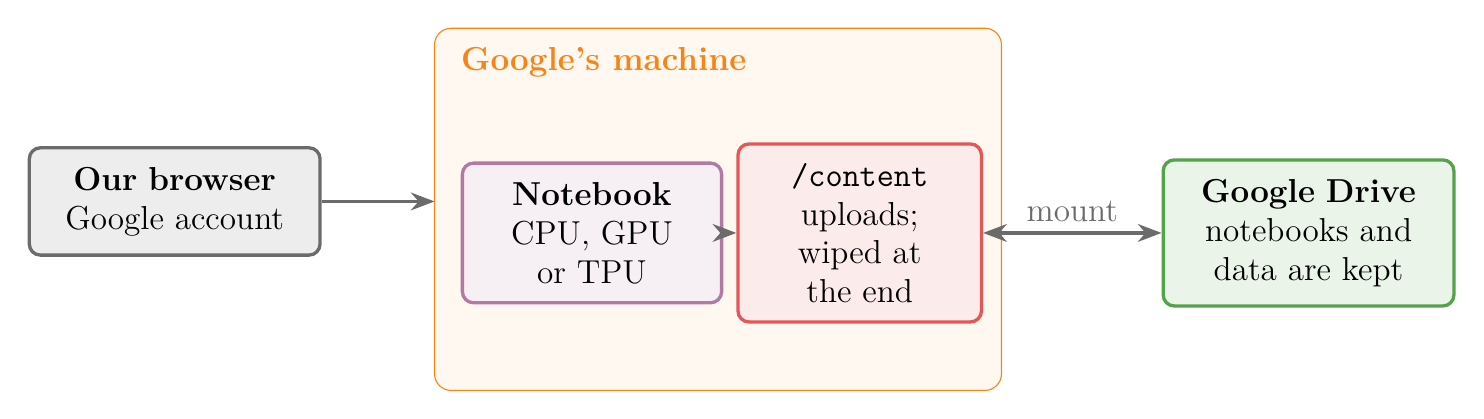
\begin{tikzpicture}[every node/.append style={font=\sffamily\large}]
\tikzset{note/.style={font=\sffamily\large, text=cgrey, align=center}}
  \node[box=cgrey, text width=3.2cm] (u) at (0,0) {\textbf{Our browser}\\Google account};
  \begin{scope}[on background layer]
    \fill[corange!6, draw=corange, rounded corners=6pt] (3.3,2.2) rectangle (10.5,-2.4);
  \end{scope}
  \node[font=\sffamily\bfseries\large, text=corange, anchor=north west] at (3.5,2.1) {Google's machine};
  \node[box=cpurple, text width=2.8cm] (n) at (5.3,-0.4) {\textbf{Notebook}\\CPU, GPU\\or TPU};
  \node[box=cred, text width=2.6cm] (c) at (8.7,-0.4) {\texttt{/content}\\uploads;\\wiped at the end};
  \node[box=cgreen, text width=3.2cm] (d) at (14.4,-0.4) {\textbf{Google Drive}\\notebooks and\\data are kept};
  \draw[arrow] (u) -- (3.3,0);
  \draw[arrow] (n) -- (c);
  \draw[arrow, {Stealth[length=3mm]}-{Stealth[length=3mm]}] (c) -- node[above, note] {mount} (d);
\end{tikzpicture}
\end{document}
